\documentclass[11pt]{scrartcl}
\usepackage[top=2cm,bottom=2cm,left=2cm,right=2cm]{geometry}
\usepackage{amsmath,amssymb,amsfonts,bm}
\usepackage{times}
\usepackage[colorlinks,linkcolor=blue,citecolor=blue,urlcolor=blue]{hyperref}
\usepackage{graphicx}
\title{Constraining the contamination in test samples}
\author{Peter Melchior}
\renewcommand*{\titlepagestyle}{empty}
\pagestyle{empty}

\begin{document}
\maketitle

A common problem in quality control is to assess the amount of contamination in a given set of samples, ideally without testing the whole. For this derivation, we will call success if the sample shows the trait it is supposed to exhibit, and contamination the absence thereof.

Using the hypergeometric distribution, we get get the probability of $k$ successful results in $n$ tests (without replacement) of a sample of size $N$, which contains a total of $K$ successful samples,
\begin{equation}
p(k | K,n,N) = \frac{\binom{K}{k}\binom{K-N}{k-n}}{\binom{N}{n}}.
\end{equation}
Since we do not vary the parameters of the test $n$ and $N$, we drop them unless important for the argument. This probability is not immediately useful since we don't know $K$ for any given sample. In absence of other information, we have to treat each possible value of $K$ equally likely,
\begin{equation}
\label{eq:pK}
p(k) = \sum_{K\in \mathcal{A}} p(k | K),
\end{equation}
where $\mathcal{A}$ denotes the set of all possible values $K$ consistent with the given test.\footnote{With this definition, \autoref{eq:pK} is not normalized to unity, but this will not matter in the following.}
Given that we have found $k$ successes in $n$ tests, the minimum number of successful samples is $k$, whereas the maximum number is $N-(n-k)$. Therefore,
\begin{equation}
\mathcal{A} = \lbrace k, k + 1, \dotsc, N-(n-k)\rbrace.
\end{equation}
Since we want to find a statement about the maximum contamination consistent with the test results, we introduce a lower bound on the success fraction $\tfrac{K}{N} \geq s$, which eliminates from the $\mathcal{A}$ all values smaller then $sN$. We then get the probability of finding $k$ successful test results under the given constraint on the success fraction $s$ of the sample as
\begin{equation}
p(k | K/N\geq s) = \sum_{K\in \mathcal{S}} p(k | K)
\end{equation}
with $\mathcal{S} = \lbrace{k_s, k_s+1, \dotsc, N-(n-k)\rbrace}$. The lower cut-off $k_s = \max(k, \lceil sN\rceil)$ makes use of the nearest integer that is not smaller than $sN$ as a conservative choice. We now invoke Bayes Theorem to relate the unknown success fraction to the measured number of successes,
\begin{equation}
p(K/N\geq s | k) = \frac{p(k | K/N\geq s)}{p(k)} = \frac{\sum_{K\in \mathcal{S}} p(k | K)}{\sum_{K\in \mathcal{A}} p(k | K)},
\end{equation}
where we exploited that the prior $p(K/N\geq s)$ is already absorbed in the definition of $\mathcal{S}$. The last equation shows that the probability of the sample success rate being at least $s$ is given by  the probability of testing samples with a sufficiently high success rate compared to the probability of testing any sample consistent with the test result $k$. A lower bound on the success rate with some confidence $c$ is given by
\begin{equation}
s(c) = \max_s \big[p(K/N\geq s | k) > c\big].
\end{equation}
A reasonable confidence in the context of many applications is $c=0.95$, which means that from 100 identical but independent experiments with test results all equal to $k$, only 5 would have an actual success rate lower than the one determined here.

Finally, the contamination rate is the complement of the success rate, therefore $1-s(c)$ is the maximum contamination rate compatible with the test result at the given level of confidence.

\section*{Required test size}
So far, we assumed a fixed set of test parameters $(k,n,N)$ for the case when the experiment is already done. Using the derivation above, we can also find the test size $n$ needed to increase the lower limit on the success fraction to some desired value $s_\textrm{min}$. This only makes sense if we assume -- prior to conducting the experiment -- that all the tests are successful and we want to know the lowest possible success rate (or highest possible contamination rate) of actual sample that is still consistent with the perfect test results. Setting $k=n$, we can then find
\begin{equation}
n_\textrm{min} = \min_n \big[ s(c) \geq s_\textrm{min} \big].
\end{equation}
We decided to accept a case where $s(c) = s_\textrm{min}$ since the numerical accuracy with which we can find $s(c)$ is limited for finite sample sizes. Otherwise, we would require a higher number of tests to be performed without any gain in statistical confidence of the actual sample success rate. This behavior is demonstrated below.

\section*{Examples \& Limitations}

Let's assume a sample of size $N=44$, for which we perform $n=10$ tests, all of which are successful. That means, $\mathcal{A}=\lbrace 10,\dotsc,44\rbrace$, and $p(k) = 4.1$. The probability of that result $k=10$ under the assumption of a underlying success rate $s$ is shown as blue line in the left panel of \autoref{fig}. If we require a confidence limit of $c=0.95$ (the horizontal dotted line), we get $s(c=0.95) = 0.79$ for the minimum success fraction (left vertical dotted line), or a maximum contamination of 21\% at 95\% confidence. 

It is apparently not possible to derive a higher success rate at that confidence level with the number of tests conducted so far, but we can increase the number of tests $n$. The right panel of \autoref{fig} shows the minimum number of tests to reach $s_\textrm{min}=0.95\ (0.90)$ as green (blue) line for a given sample size $N$. We can read off that for $N=44$, we need to test $n_\textrm{min}=27$ samples successfully to make sure that the maximum contamination rate is below 5\% at 95\% confidence. This is demonstrated by the green line in the left panel. What should become clear from the right panel is that for small samples sizes $N$, a proportionally large number of tests have to be performed to reach any relevant $s_\textrm{min}$, which becomes increasingly impractical if untested samples are to remain for later studies.

Some oddities are worthwhile mentioning: As a direct consequence of demanding an integer number $k_s$, a range of values of $s$ yield the same $p(K/N\geq s | k)$. Another counter-intuitive result of this rounding error is that $n_\textrm{min}$ is not a monotonic function of $N$, but exhibits jumps whenever $\lceil s_\textrm{min}N\rceil$ increases by 1. Both of these limitations are visible in \autoref{fig}.

\begin{figure}
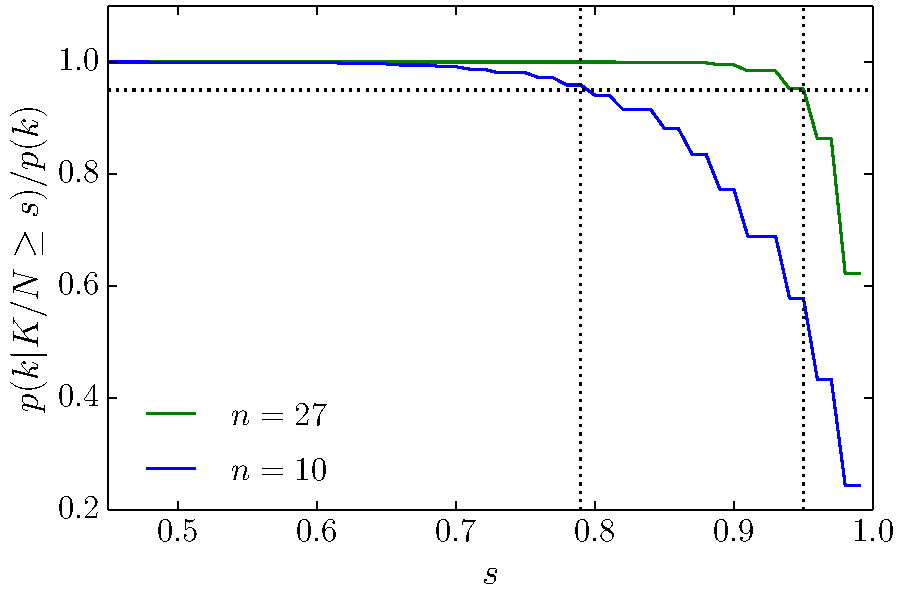
\includegraphics[width=0.5\linewidth]{probKGivenS}
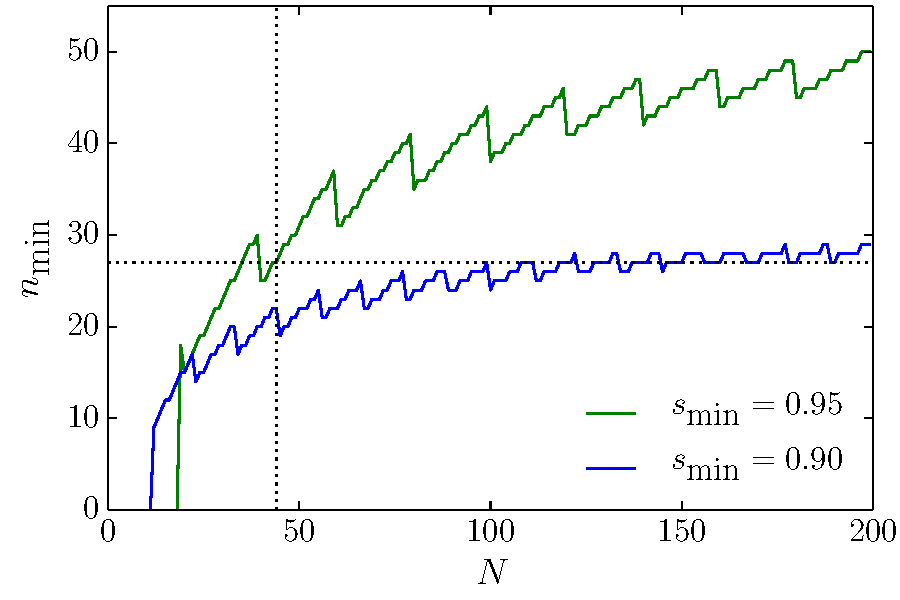
\includegraphics[width=0.5\linewidth]{n_min}
\caption{\emph{Left}: Probability of a sample exceeding the success rate $s$ given $k=n$ successful tests.\newline
\emph{Right}: Minimum test length to confirm a minimum success rate $s\geq s_\textrm{min}$ at 95\% confidence level.}
\label{fig}
\end{figure}

\subsection*{Code}
The python code for performing the aforementioned calculations can be found at \url{https://github.com/pmelchior/test-sample-contamination}.

\end{document}
